% main.tex -- PRL-style manuscript (REVTeX 4.2). Direction 11, iteration 5.
% ALL device numbers are SIMULATION / design predictions (sources: ../data/iter5_final.json,
% ../data/iter5_power_sweep.csv, ../data/iter5_Q_sweep.csv, ../data/key_results.json, ./eo_baseline.json).
% Literature numbers: see per-entry verification comments in refs.bib.
\documentclass[aps,prl,reprint,superscriptaddress,amsmath,amssymb,floatfix]{revtex4-2}
\usepackage{graphicx}
\usepackage{bm}
\usepackage[colorlinks=true,linkcolor=blue,citecolor=blue,urlcolor=blue]{hyperref}
\newcommand{\etash}{\eta_{\rm shift}}
\newcommand{\etaabs}{\eta_{\rm abs}}

\begin{document}

\title{Microwatt-driven frequency shifting in an acoustically modulated thin-film lithium niobate photonic molecule: a simulation study}

\author{Xinlei Chen}
\affiliation{Affiliation to be added}
% TODO: author list / affiliations / acknowledgements to be completed by the group.

\date{\today}

\begin{abstract}
Coupled-ring (``photonic molecule'') electro-optic frequency shifters on thin-film lithium niobate (TFLN) shift $\sim$99\% of the output light but need $\sim$0.1~W of microwave drive. We show by simulation that the same architecture driven by an interdigital-transducer (IDT) acoustic resonator, which modulates only one ring over part of its circumference, can reach the same shift efficiency with microwatt-level drive. We solve the full time-domain coupled-mode equations without the rotating-wave approximation. We take the acousto-optic drive strength from published resonant half-wave-voltage--length products. A non-suspended design at 0.842~GHz shifts 99.2\% of the output light with 79~$\mu$W of RF power. A suspended design at 3.33~GHz shifts 98.4\% with 7.2~$\mu$W. The measured electro-optic device needs 96~mW for 98.7\%, so the required RF power is $\sim$1{,}200--13{,}000 times lower. Most of this reduction in the non-suspended design comes from the narrower optical linewidth that a sub-GHz shift allows. An electro-optic drive with the same optical parameters would need $\sim$95~$\mu$W. The acoustic resonance itself contributes a large gain ($\approx$475$\times$) only in the suspended design. The predictions rely on a linear extrapolation of the acousto-optic coupling to partial ring coverage, which has not been verified experimentally. They also assume intrinsic quality factors $Q_i\gtrsim10^7$. The cost is a fixed shift frequency, a narrow RF bandwidth (132.5~MHz and $\sim$1~MHz), and a 1.8~dB insertion loss compared with 0.45~dB measured for the electro-optic device.
\end{abstract}

\maketitle

% ---------------------------------------------------------------- Introduction
\emph{Introduction.}---Encoding photonic qubits in discrete frequency bins requires low-loss, coherent devices that move photons between bins~\cite{Lukens2017,Kues2017,Lu2018}. TFLN supports such devices because it combines strong Pockels, piezoelectric, and photoelastic responses with ultralow-loss resonators~\cite{Wang2018,Zhang2017,Zhu2026loss}. Recent TFLN demonstrations include single-photon spectral shearing over $\pm641$~GHz~\cite{Zhu2022}, an integrated quantum frequency processor~\cite{Yang2026}, and coupled-cavity frequency beam splitters~\cite{Cohen2026}. The coupled-ring frequency shifter of Hu \emph{et al.}~\cite{Hu2021} is the benchmark for single-tone shifting. Its microwave drive hybridizes the symmetric (S) and antisymmetric (AS) supermodes of a photonic molecule~\cite{Zhang2019}. When the coupling rates satisfy a generalized critical-coupling condition, the light is transferred in one direction between the two supermodes. The device shifts 98.7\% of the output light by 28.2~GHz with 0.45~dB insertion loss (IL), and 99.1\% (up) and 99.4\% (down) at 12.5~GHz~\cite{Hu2021}. It needs 96~mW of microwave power (3.1~V peak at the 50-$\Omega$ probe). The authors project that 1~V ($\approx$10~mW) would suffice at $Q_i\sim10^7$~\cite{Hu2021}. For many-channel or cryogenic frequency-domain processors, this drive power sets the heat load.

Acoustic resonators on TFLN boost the microwave-to-optical phase modulation through resonance. A suspended 100-$\mu$m resonator at 3.33~GHz gives $V_\pi=4.6$~V ($V_\pi L=0.046$~V\,cm, one arm modulated)~\cite{Shao2019}. A non-suspended push-pull modulator gives $V_\pi L=1.004$~V\,cm at 0.842~GHz with a 132.5~MHz bandwidth~\cite{Ni2026}. Acoustic waves have also been used to modulate integrated resonators~\cite{Tadesse2014} and to control a photonic molecule dynamically~\cite{Kapfinger2015}. An optomechanical single-photon frequency shifter with near-unity efficiency has also been demonstrated~\cite{Fan2016}. % TODO(verify): Fan2016 checked against abstract only; keep qualitative.
TFLN acousto-optic frequency shifters based on traveling-wave deflection, however, reach only 3.5\% on-chip efficiency at 30~dBm~\cite{Shao2020}. Here we ask a narrower question: what happens if the acoustic resonator replaces the electrodes of the Hu architecture? All device numbers below come from simulation and are not measurements.

% ---------------------------------------------------------------- Model
\emph{Model.}---We follow Eq.~(S2) of Ref.~\cite{Hu2021}. Two identical rings (amplitudes $a_{1,2}$) couple to each other at rate $\mu$, and ring~1 couples to the bus waveguide at rate $\gamma$. Both rings have intrinsic loss $\kappa_i$. Only ring~1 sits in the acoustic field, so its resonance is modulated as $\delta\omega\cos\Omega_m t$:
\begin{align}
\dot a_1&=\Big[-i\big(\Delta+\delta\omega\cos\Omega_m t\big)-\tfrac{\gamma+\kappa_i}{2}\Big]a_1-i\mu a_2-\sqrt{\gamma}\,\alpha_{\rm in},\nonumber\\
\dot a_2&=\Big[-i\Delta-\tfrac{\kappa_i}{2}\Big]a_2-i\mu a_1,\qquad a_{\rm out}=\alpha_{\rm in}+\sqrt{\gamma}\,a_1 .
\label{eq:eom}
\end{align}
The laser is tuned to the S mode ($\Delta=\mu$), and the doublet splitting is matched to the acoustic frequency, $2\mu=\Omega_m$. We integrate Eq.~\eqref{eq:eom} directly with a fourth-order Runge--Kutta scheme (80 steps per acoustic period) and make no rotating-wave approximation. We then project $a_{\rm out}$, averaged over the final 20~ns, onto the frequencies $\omega_L+q\Omega_m$ ($|q|\le3$). In the S/AS basis the single-ring term becomes $\tfrac{\delta\omega}{2}\cos\Omega_m t\,(c_S^\dagger c_S+c_A^\dagger c_A+c_S^\dagger c_A+{\rm h.c.})$. The coupling between the two supermodes is therefore $\delta\omega/2$, half the push-pull value, and the critical condition becomes $\delta\omega\simeq\gamma$ for $\kappa_i\ll\gamma$. We define the efficiencies as in Ref.~\cite{Hu2021}: $\etash=P_{\rm shift}/P_{\rm out}$, $\etaabs=P_{\rm shift}/P_{\rm in}$, and ${\rm IL}=-10\log_{10}(P_{\rm out}/P_{\rm in})$.

We calibrate the acoustic drive from the measured MZI modulators. A peak voltage $V$ at a 50-$\Omega$ source ($P_{\rm RF}=V^2/2R$) produces a single-pass phase $\Delta\phi=\pi V L_a/(V_\pi L)_{\rm 1arm}$ over the acoustically covered length $L_a$. This phase shifts the ring resonance by
\begin{equation}
\delta\omega=\Delta\phi\,\frac{c}{n_g L_{\rm ring}},\qquad n_g=2.3 .
\label{eq:cal}
\end{equation}
Design~A (non-suspended) uses Ref.~\cite{Ni2026}. Converting push-pull to single-arm modulation doubles the reported value to $(V_\pi L)_{\rm 1arm}=2.008$~V\,cm, at $\Omega_m/2\pi=0.842$~GHz with $L_a=400~\mu$m and $L_{\rm ring}=1.2$~mm (coverage 33\%). Design~B (suspended) uses the single-arm MZI of Ref.~\cite{Shao2019}: 0.046~V\,cm at 3.33~GHz, with $L_a=100~\mu$m and $L_{\rm ring}=0.667$~mm (coverage 15\%). Equation~\eqref{eq:cal} then gives $\delta\omega/2\pi=1.08$~GHz/V (A) and 21.3~GHz/V (B). Table~\ref{tab:main} lists the optical parameters. Both designs keep $\kappa_i/\gamma=0.1$ and stay in the sideband-resolved regime, with $\Omega_m\gg\gamma/2+\kappa_i$.

\begin{figure*}[t]
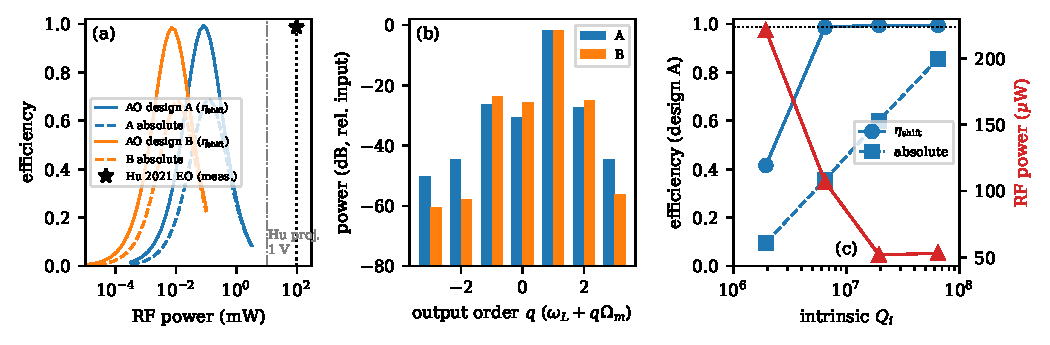
\includegraphics[width=\textwidth]{figures/fig5_ao_molecule.pdf}
\caption{Acoustically driven photonic-molecule shifter (simulation). (a)~Shift efficiency $\etash$ (solid) and absolute efficiency $\etaabs$ (dashed) versus RF power for design~A (blue, 0.842~GHz, non-suspended) and design~B (orange, 3.33~GHz, suspended). The star marks the measured EO device of Ref.~\cite{Hu2021} (98.7\%, 96~mW; dotted line). The dash-dotted line marks the authors' projected 1~V ($\approx$10~mW) drive. (b)~Output power in each order $q$ (frequency $\omega_L+q\Omega_m$), relative to the input, at the optimum drive. Order $q=+1$ is the shifted line. (c)~Design~A versus intrinsic $Q_i$: $\etash$ (circles), $\etaabs$ (squares), and the required RF power (triangles, right axis). At each $Q_i$, $\gamma$ and $\delta\omega$ are re-optimized, so these points differ slightly from the operating point in Table~\ref{tab:main}. The dotted line marks 98.7\%.}
\label{fig:main}
\end{figure*}

% ---------------------------------------------------------------- Results
\emph{Results.}---Figure~\ref{fig:main}(a) shows the typical frequency-beam-splitter behavior: $\etash$ rises from zero to a maximum as the drive increases. The maximum lies at $\delta\omega/2\pi=96$~MHz (A) and 570~MHz (B), close to the predicted $\delta\omega\simeq\gamma$. Design~A reaches $\etash=99.2\%$ at $P_{\rm RF}=79~\mu$W (89~mV peak). Design~B reaches $\etash=98.4\%$ at $7.2~\mu$W (27~mV peak). Table~\ref{tab:main} compares both designs with the measured EO device~\cite{Hu2021}. At equal or slightly better $\etash$, the drive power is $1.2\times10^3$ (A) to $1.3\times10^4$ (B) times lower than the measured 96~mW. It is also 2--3 orders of magnitude below the authors' projected 1~V case. In both designs about a third of the input power is lost: IL is 1.8~dB and $\etaabs=66\%$ (A) and 65\% (B). The measured EO device reaches IL $=0.45$~dB and $\etaabs\approx0.987\times10^{-0.045}\approx89\%$.

The output spectrum [Fig.~\ref{fig:main}(b)] shows the cost of driving a single ring. The common-mode term $\tfrac{\delta\omega}{2}(c_S^\dagger c_S+c_A^\dagger c_A)$ phase-modulates both supermodes, which generates parasitic orders. Relative to the shifted line, the largest parasitic order is $-24.6$~dB in A ($q=-1$; $q=+2$ is at $-25.6$~dB) and $-21.7$~dB in B ($q=-1$). The residual carrier is at $-28.7$~dB (A) and $-23.7$~dB (B). For HOM-type quantum interference these orders must be filtered. The shift is a linear, coherent transformation driven by a classical tone, as in Ref.~\cite{Hu2021}. We did not separately simulate the HOM visibility or the thermal-phonon phase noise of the acoustic drive for this design.

\begin{table}[b]
\caption{Operating points (simulation) compared with the measured EO shifter~\cite{Hu2021}. $Q_i=\omega/\kappa_i$ at $\omega/2\pi=193.4$~THz for designs A and B.}
\label{tab:main}
\begin{ruledtabular}
\small
\begin{tabular}{lccc}
 & A (sim.) & B (sim.) & Hu~\cite{Hu2021} (meas.)\\
\hline
$\Omega_m/2\pi$ (GHz) & 0.842 & 3.33 & 28.2\\
Drive & AO, non-susp. & AO, susp. & EO\\
Calibration & \cite{Ni2026} & \cite{Shao2019} & ---\\
$\gamma/2\pi$ (GHz) & 0.10 & 0.60 & 5.31\\
$\kappa_i/2\pi$ (MHz) & 10 & 60 & 170\\
$Q_i$ & $1.9\times10^7$ & $3.2\times10^6$ & $1.1\times10^6$\\
$\etash$ & 99.2\% & 98.4\% & 98.7\%\\
Peak voltage & 89~mV & 27~mV & 3.1~V\\
$P_{\rm RF}$ & 79~$\mu$W & 7.2~$\mu$W & 96~mW\\
IL (dB) & 1.8 & 1.8 & 0.45\\
$\etaabs$ & 66\% & 65\% & $\approx$89\%\\
Max.\ spur (dB) & $-24.6$ & $-21.7$ & ---\\
RF bandwidth & 132.5 MHz$^{a}$ & $\sim$1 MHz$^{a}$ & $>$3 GHz\\
\end{tabular}
\end{ruledtabular}
\raggedright\footnotesize $^{a}$Acoustic bandwidth of the calibration device~\cite{Ni2026,Shao2019}. The shifter's own RF-detuning tolerance was not simulated and is further limited by the optical linewidth $\gamma/2+\kappa_i$ (60 and 360~MHz).
\end{table}

\emph{Dependence on intrinsic $Q$.}---The power advantage depends on high intrinsic $Q$ [Fig.~\ref{fig:main}(c)]. A sub-GHz shift is sideband-resolved only if $\gamma\ll\Omega_m$, and the generalized critical-coupling condition additionally needs $\kappa_i\ll\gamma$. For design~A at $Q_i=6.4\times10^7$ we find $\etash=99.5\%$, $\etaabs=86\%$, and IL $=0.65$~dB. At $1.9\times10^7$ we find 99.5\% and 60\%; at $6.4\times10^6$, 98.7\% and 36\%. At $1.9\times10^6$, where $\kappa_i$ approaches $\gamma$, the device fails ($\etash=42\%$). Design~A therefore needs $Q_i\gtrsim10^7$, which TFLN rings already achieve: $Q_i\sim10^7$~\cite{Zhang2017}, and a most probable $\kappa_i/2\pi=10.4$~MHz in recent statistics~\cite{Zhu2026loss}. Design~B assumes $\kappa_i/2\pi=60$~MHz ($Q_i\approx3.2\times10^6$) in a suspended ring that partly overlaps the acoustic resonator. This is somewhat better than the $\kappa_i/2\pi\approx81$~MHz implied by the suspended racetrack of Ref.~\cite{Shao2019} ($\kappa/2\pi=95$~MHz, $2\kappa_e/\kappa=0.3$).

\emph{Where the advantage comes from.}---The comparison with Ref.~\cite{Hu2021} mixes two effects. Part of the reduction comes from the narrower linewidth that a sub-GHz shift permits; an EO drive would benefit from it equally. The rest comes from the higher modulation per volt of an acoustic resonance. To separate the two, we simulated a push-pull EO drive of the same optical parameters [Eq.~(S2) of Ref.~\cite{Hu2021}]. We used Hu's EO coefficient of $\sim$0.5~GHz/V and assumed that the electrode voltage equals the source voltage. With design~A's optics this EO molecule reaches $\etash=99.8\%$ at $\approx$95~$\mu$W. With design~B's optics it needs $\approx$3.4~mW. Per unit RF power, the non-suspended acoustic drive is therefore comparable to EO; nearly all of design~A's advantage over the measured device comes from operating at a lower frequency with a narrower linewidth. The suspended resonator (B) gives $\approx$20$\times$ more supermode coupling per volt and $\approx$475$\times$ less power at matched optics. A low-frequency EO electrode that delivers more than the source voltage would weaken the case for design~A further. We did not model the electrode circuit.

% ---------------------------------------------------------------- Limitations
\emph{Limitations.}---These results are design predictions with the following caveats.
(i)~\emph{Drive strength.} We obtain $\delta\omega$ by extrapolating the published resonant $V_\pi L$~\cite{Ni2026,Shao2019} linearly to a ring that the acoustic field covers only partially (33\% and 15\%). This assumes the same IDT efficiency, acousto-optic mode overlap, and uniform acoustic phase along the covered section as in the MZI calibrations. The extrapolation needs experimental verification. The value $n_g=2.3$ is also assumed.
(ii)~\emph{Fixed frequency, narrow bandwidth.} The shift frequency is set by the acoustic resonance (0.842 or 3.33~GHz). The RF bandwidth is limited to that of the acoustic device, 132.5~MHz for A~\cite{Ni2026} and $\sim$1~MHz for B~\cite{Shao2019}. Ref.~\cite{Hu2021} reaches 11--28.2~GHz with $>3$~GHz bandwidth. The doublet splitting must also match $\Omega_m$ to well within the optical linewidth, which requires thermal tuning.
(iii)~\emph{Loss.} IL is 1.8~dB versus 0.45~dB measured in Ref.~\cite{Hu2021}, so our absolute efficiency is lower (66\% vs $\approx$89\%). It becomes comparable only at $Q_i\gtrsim6\times10^7$.
(iv)~\emph{Quality factor.} The power advantage requires $Q_i\gtrsim10^7$ (design A).
(v)~\emph{Not modeled.} We did not simulate optical loss from the IDT metal or the acoustic resonator, acoustic heating, or the resulting thermo-optic drift. Ref.~\cite{Shao2019} observed a heating-induced red shift at mW drive. Our drives are at the $\mu$W level, but we have not modeled this effect.
(vi)~\emph{Model provenance of the supporting routes.} The phononic 90$^\circ$ hybrid used for the IQ route (Supplemental Material) is our reconstruction of the group's acoustic-MZI model from its governing equations, since no code was available. Its acoustic parameters are borrowed from GaN-on-sapphire~\cite{Xu2025} and have not been re-derived for LN. The main result does not depend on this model.

\emph{Routes not pursued.}---We also simulated three other acoustic routes (Supplemental Material), and none outperforms published devices. An acoustically driven IQ single-sideband shifter is limited by the Bessel function to 33.9\% efficiency. A phase-matched intermodal shifter would need $\sim$70~W for complete conversion at the calibration of Ref.~\cite{Shao2020}. Cavity-enhanced microwave-to-optical designs fall short of cryogenic demonstrations~\cite{Weaver2024,Jiang2023,Warner2025,Mirhosseini2020}. These results motivated the resonant photonic-molecule design presented here.

\emph{Conclusion.}---In simulation, replacing the EO drive of a TFLN photonic-molecule shifter with an IDT acoustic resonator keeps $\etash\approx99\%$ while reducing the RF power from 96~mW (measured EO) to 79~$\mu$W (non-suspended) or 7.2~$\mu$W (suspended). In return, the device becomes fixed-frequency and narrowband and has higher loss. The resonant acoustic enhancement itself matters mainly in the suspended design. The key experimental tests are the acousto-optic coupling of a partially covered high-$Q$ ring and the optical loss and heating added by the IDT.

\bibliography{refs}

% ================================================================ Supplement
\clearpage
\onecolumngrid
\begin{center}\textbf{\large Supplemental Material}\end{center}
\setcounter{figure}{0}\renewcommand{\thefigure}{S\arabic{figure}}
\setcounter{table}{0}\renewcommand{\thetable}{S\arabic{table}}
\setcounter{equation}{0}\renewcommand{\theequation}{S\arabic{equation}}

The routes below are supporting material. None of them beats published results; they explain why the main text uses the resonant photonic molecule. All numbers come from simulation (\texttt{data/key\_results.json}).

\emph{S1. Acoustic IQ single-sideband shifter.} We used a 50:50 acoustic directional coupler as a phononic 90$^\circ$ hybrid; its two output ports differ by $-90.0^\circ$, as verified numerically. The two outputs drive the I and Q push-pull sub-MZIs of a nested optical IQ modulator. The model is reconstructed from equations, with GaN parameters~\cite{Xu2025}: coupler full-transfer length 79.14~$\mu$m, thermo-acoustic phase 4.03~rad/W, and 2.4~dB/mm acoustic loss. The reconstructed DC--arm--DC model reproduces $T=\tfrac12[1+\cos(\alpha P_H+\phi_0)]$ to within $4\times10^{-16}$. The ideal shifted-sideband power is $J_1^2(\Delta\phi/2)$, with a maximum of 33.9\% at $\Delta\phi=3.68$~rad (unfiltered HOM visibility 0.969). Requiring a visibility of 0.99 lowers the efficiency to 30.1\%. With the calibration of Ref.~\cite{Ni2026}, maximum efficiency needs 19.3~W at $L=400~\mu$m or 0.77~W at $L=2$~mm (Fig.~\ref{fig:s1}). The measured EO photonic molecule reaches 98.7--99.4\%~\cite{Hu2021}.

\begin{figure}[h]
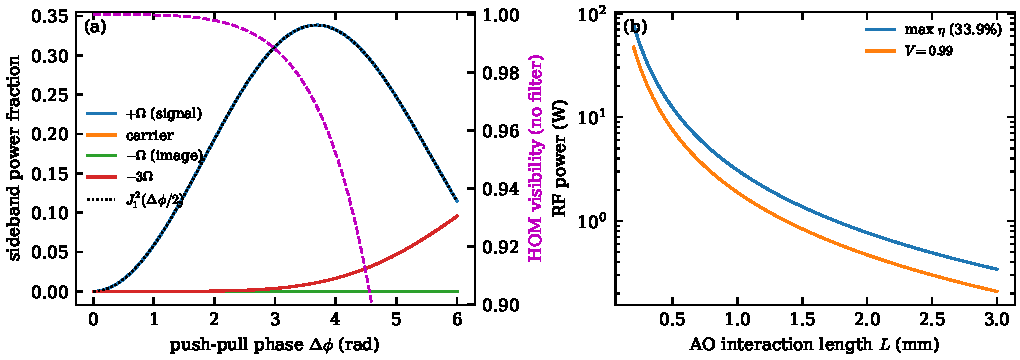
\includegraphics[width=0.75\textwidth]{figures/fig1_ssb_iq.pdf}
\caption{IQ single-sideband route. (a)~Sideband powers and unfiltered HOM visibility versus push-pull phase. (b)~Required RF power versus acousto-optic interaction length.}
\label{fig:s1}
\end{figure}

\emph{S2. Fabrication tolerance.} We ran Monte Carlo simulations (300 samples per point) of the coupler length error $\sigma_L/L$, with 0.05~rad thermal phase noise, 30~dB sub-MZI extinction, and filtering of $|n|\ge3$ orders. Without trimming, the image rejection falls from 36 to 29~dB as $\sigma_L/L$ increases from 0 to 10\%. After thermo-acoustic trimming it is 38~dB ($V=0.9997$) at 5\% and 33~dB ($V=0.9993$) at 10\%. Carrier suppression saturates near 39~dB, a limit set by the sub-MZI extinction (Fig.~\ref{fig:s2}).

\begin{figure}[h]
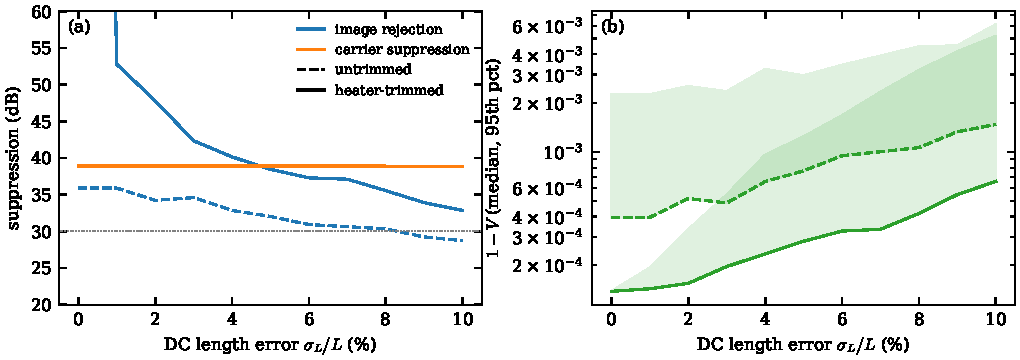
\includegraphics[width=0.75\textwidth]{figures/fig2_tolerance.pdf}
\caption{Tolerance of the IQ route to coupler length errors. (a)~Image and carrier suppression, untrimmed and heater-trimmed. (b)~HOM infidelity $1-V$.}
\label{fig:s2}
\end{figure}

\emph{S3. Phase-matched intermodal shifter.} We modeled TE$_0(\omega)\to$TE$_1(\omega+\Omega)$ conversion with coupled-mode equations, calibrated to the 3.5\% efficiency at 30~dBm of Ref.~\cite{Shao2020}. Complete lossless conversion would need about 70~W. Acoustic loss of 1--2.4~dB/mm lowers the achievable efficiency further (Fig.~\ref{fig:s3}).

\begin{figure}[h]
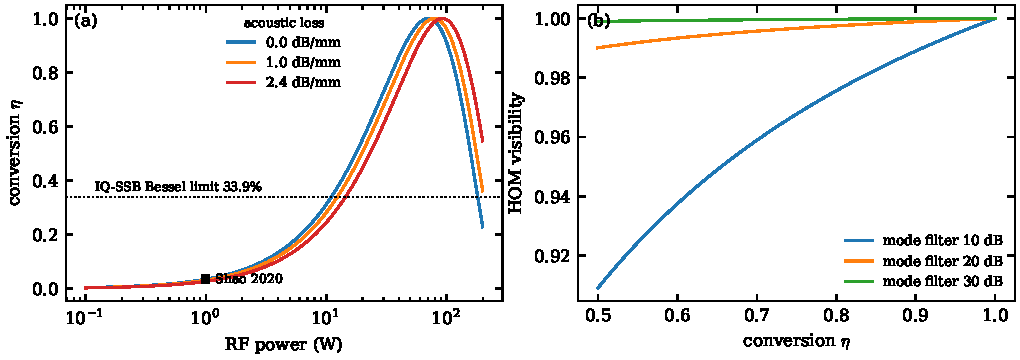
\includegraphics[width=0.75\textwidth]{figures/fig3_intermodal.pdf}
\caption{Intermodal route. (a)~Conversion efficiency versus RF power for several acoustic losses. (b)~HOM visibility versus conversion efficiency for different mode-filter extinctions.}
\label{fig:s3}
\end{figure}

\emph{S4. Microwave-to-optical conversion.} The linearized model of Ref.~\cite{Shao2019} with its Table~S2 parameters reproduces the published single-photon cooperativity, $C_0=3.98\times10^{-8}$ ($4\times10^{-8}$ published), and efficiency, $\eta=1.78\times10^{-5}$ at 1~mW (0.0017\% published). We then considered three hypothetical designs. Double resonance gives 1.8\% at 1~mW. Critically coupled optics and IDT give 25\%. Overcoupled optics and IDT ($\kappa_e/\kappa=\gamma_e/\gamma=0.9$) give 74\% at 1~mW, with a maximum of 81\%. The added noise of the overcoupled design is 346 quanta at 300~K and 0.069 at 0.1~K. This room-temperature model does not compete with cryogenic demonstrations~\cite{Weaver2024,Jiang2023,Warner2025,Mirhosseini2020} (Fig.~\ref{fig:s4}).

\begin{figure}[h]
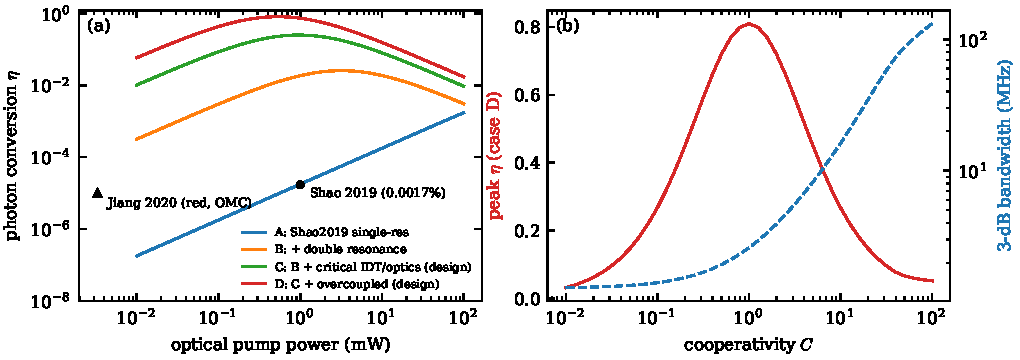
\includegraphics[width=0.75\textwidth]{figures/fig4_transducer.pdf}
\caption{Microwave-to-optical route. (a)~Photon conversion efficiency versus optical pump power. (b)~Peak efficiency and bandwidth versus cooperativity for the overcoupled design.}
\label{fig:s4}
\end{figure}

\emph{S5. Matched EO baseline.} The baseline uses Eq.~(S2) of Ref.~\cite{Hu2021} with push-pull modulation $\pm\Omega\cos\Omega_m t$ on both rings, Hu's coefficient of $\sim$0.5~GHz/V on the capacitor~\cite{Hu2021}, the source voltage applied directly to the electrode, and $P=V^2/(2\cdot50~\Omega)$. Design~A's optics give $\Omega/2\pi=49$~MHz, $V=97.5$~mV, $\approx95~\mu$W, and $\etash=99.8\%$. Design~B's optics give $\Omega/2\pi=292$~MHz, $V=0.585$~V, $\approx3.4$~mW, and $\etash=99.8\%$ (\texttt{paper/eo\_baseline.py}). Push-pull driving cancels the common-mode term, which explains the higher $\etash$.

\begin{table}[h]
\caption{Selected literature benchmarks and how each was verified.}
\begin{ruledtabular}
\begin{tabular}{p{4.2cm}p{6.6cm}p{5.4cm}}
Work & Reported metric (measured) & Verification\\
\hline
Hu \emph{et al.}~\cite{Hu2021} & 98.7\%, 0.45~dB, 96~mW @28.2~GHz; 99.1/99.4\% @12.5~GHz & arXiv full text + Supplement\\
Shao \emph{et al.} 2019~\cite{Shao2019} & $V_\pi=4.6$~V (100~$\mu$m), 3.33~GHz, $\sim$1~MHz & arXiv full text\\
Ni \emph{et al.}~\cite{Ni2026} & $V_\pi L=1.004$~V\,cm, 0.842~GHz, 132.5~MHz & arXiv abstract\\
Shao \emph{et al.} 2020~\cite{Shao2020} & 3.5\% @30~dBm, $>$30~dB carrier supp., 70~MHz & arXiv full text\\
Fan \emph{et al.}~\cite{Fan2016} & near-unity efficiency, up to 150~GHz (qualitative) & abstract only (TODO: full text)\\
Zhu \emph{et al.}~\cite{Zhu2022} & $\pm641$~GHz shearing of single photons & abstract\\
Weaver \emph{et al.}~\cite{Weaver2024} & 0.9\%, 14.8~MHz & abstract\\
Jiang \emph{et al.}~\cite{Jiang2023} & 5\% continuous conversion & abstract\\
Warner \emph{et al.}~\cite{Warner2025} & up to 1.18\% & abstract\\
\end{tabular}
\end{ruledtabular}
\end{table}

\end{document}
